
\chapter{Analyse}
\section{Systembeschreibung}
\subsection{Systemarchitektur}
\begin{figure}[!ht]
  \centering
  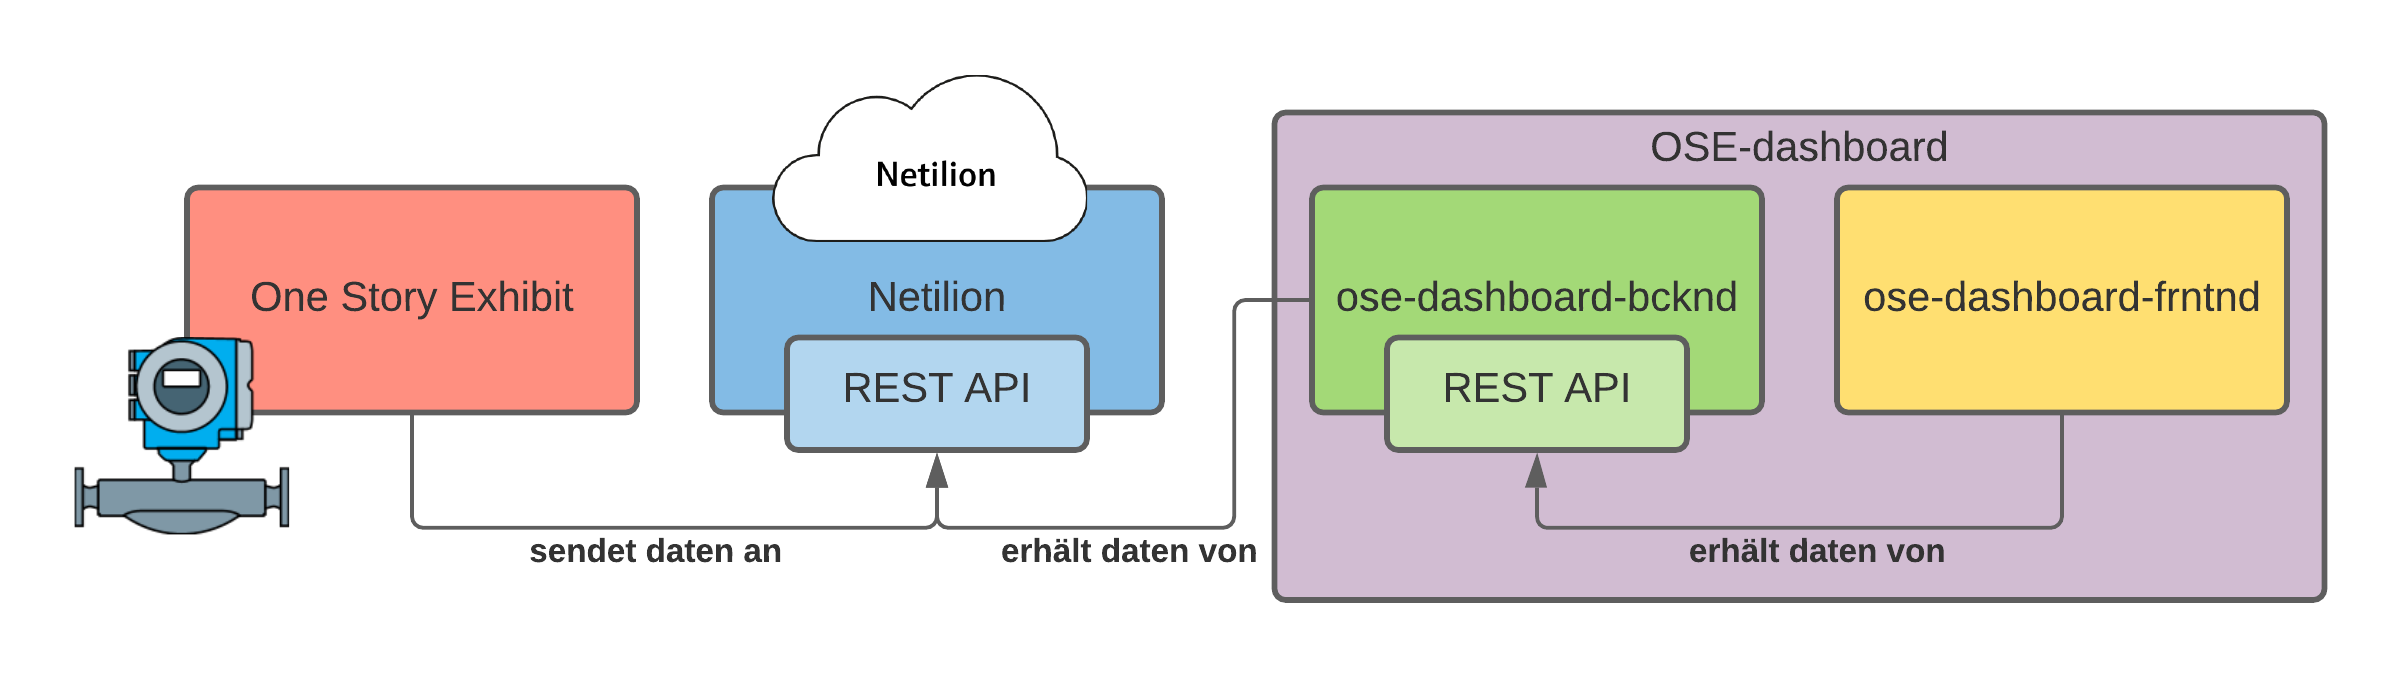
\includegraphics[width=1\linewidth]{./images/system.png}
  \caption[Eine von mir mit Lucidchart erstellte grobe Systemarchitektur]{Grobe Systemarchitektur}
  \label{fig:systemarchitektur}
\end{figure}
Das System des OSE Dashboard besteht aktuell aus vier essentiellen Teilen. Die Systemteile werden in den nachfolgenden Kapiteln \ref{arch-ose}, \ref{arch-netilion}, \ref{arch-backend} und \ref{arch-frontend} erläutert.
\subsection{One Story Exhibit} \label{arch-ose}
Die Anlage/-n deren Daten von der Applikation ausgewertet werden sollen. In diesem Projekt sind dies Ausstellungsmodelle von Endress+Hauser selbst. Die Gruppe verwendet diese an Messen oder in Verkaufsstellen, um den Kunden unser umfassendes Portfolio an Messgeräten näher zu bringen. Diese Applikation soll diesem Prozess helfen und zeigen, was mit unserem IIoT-Angebot möglich ist.
\subsection{Netilion} \label{arch-netilion}
\begin{figure}[!ht]
  \centering
  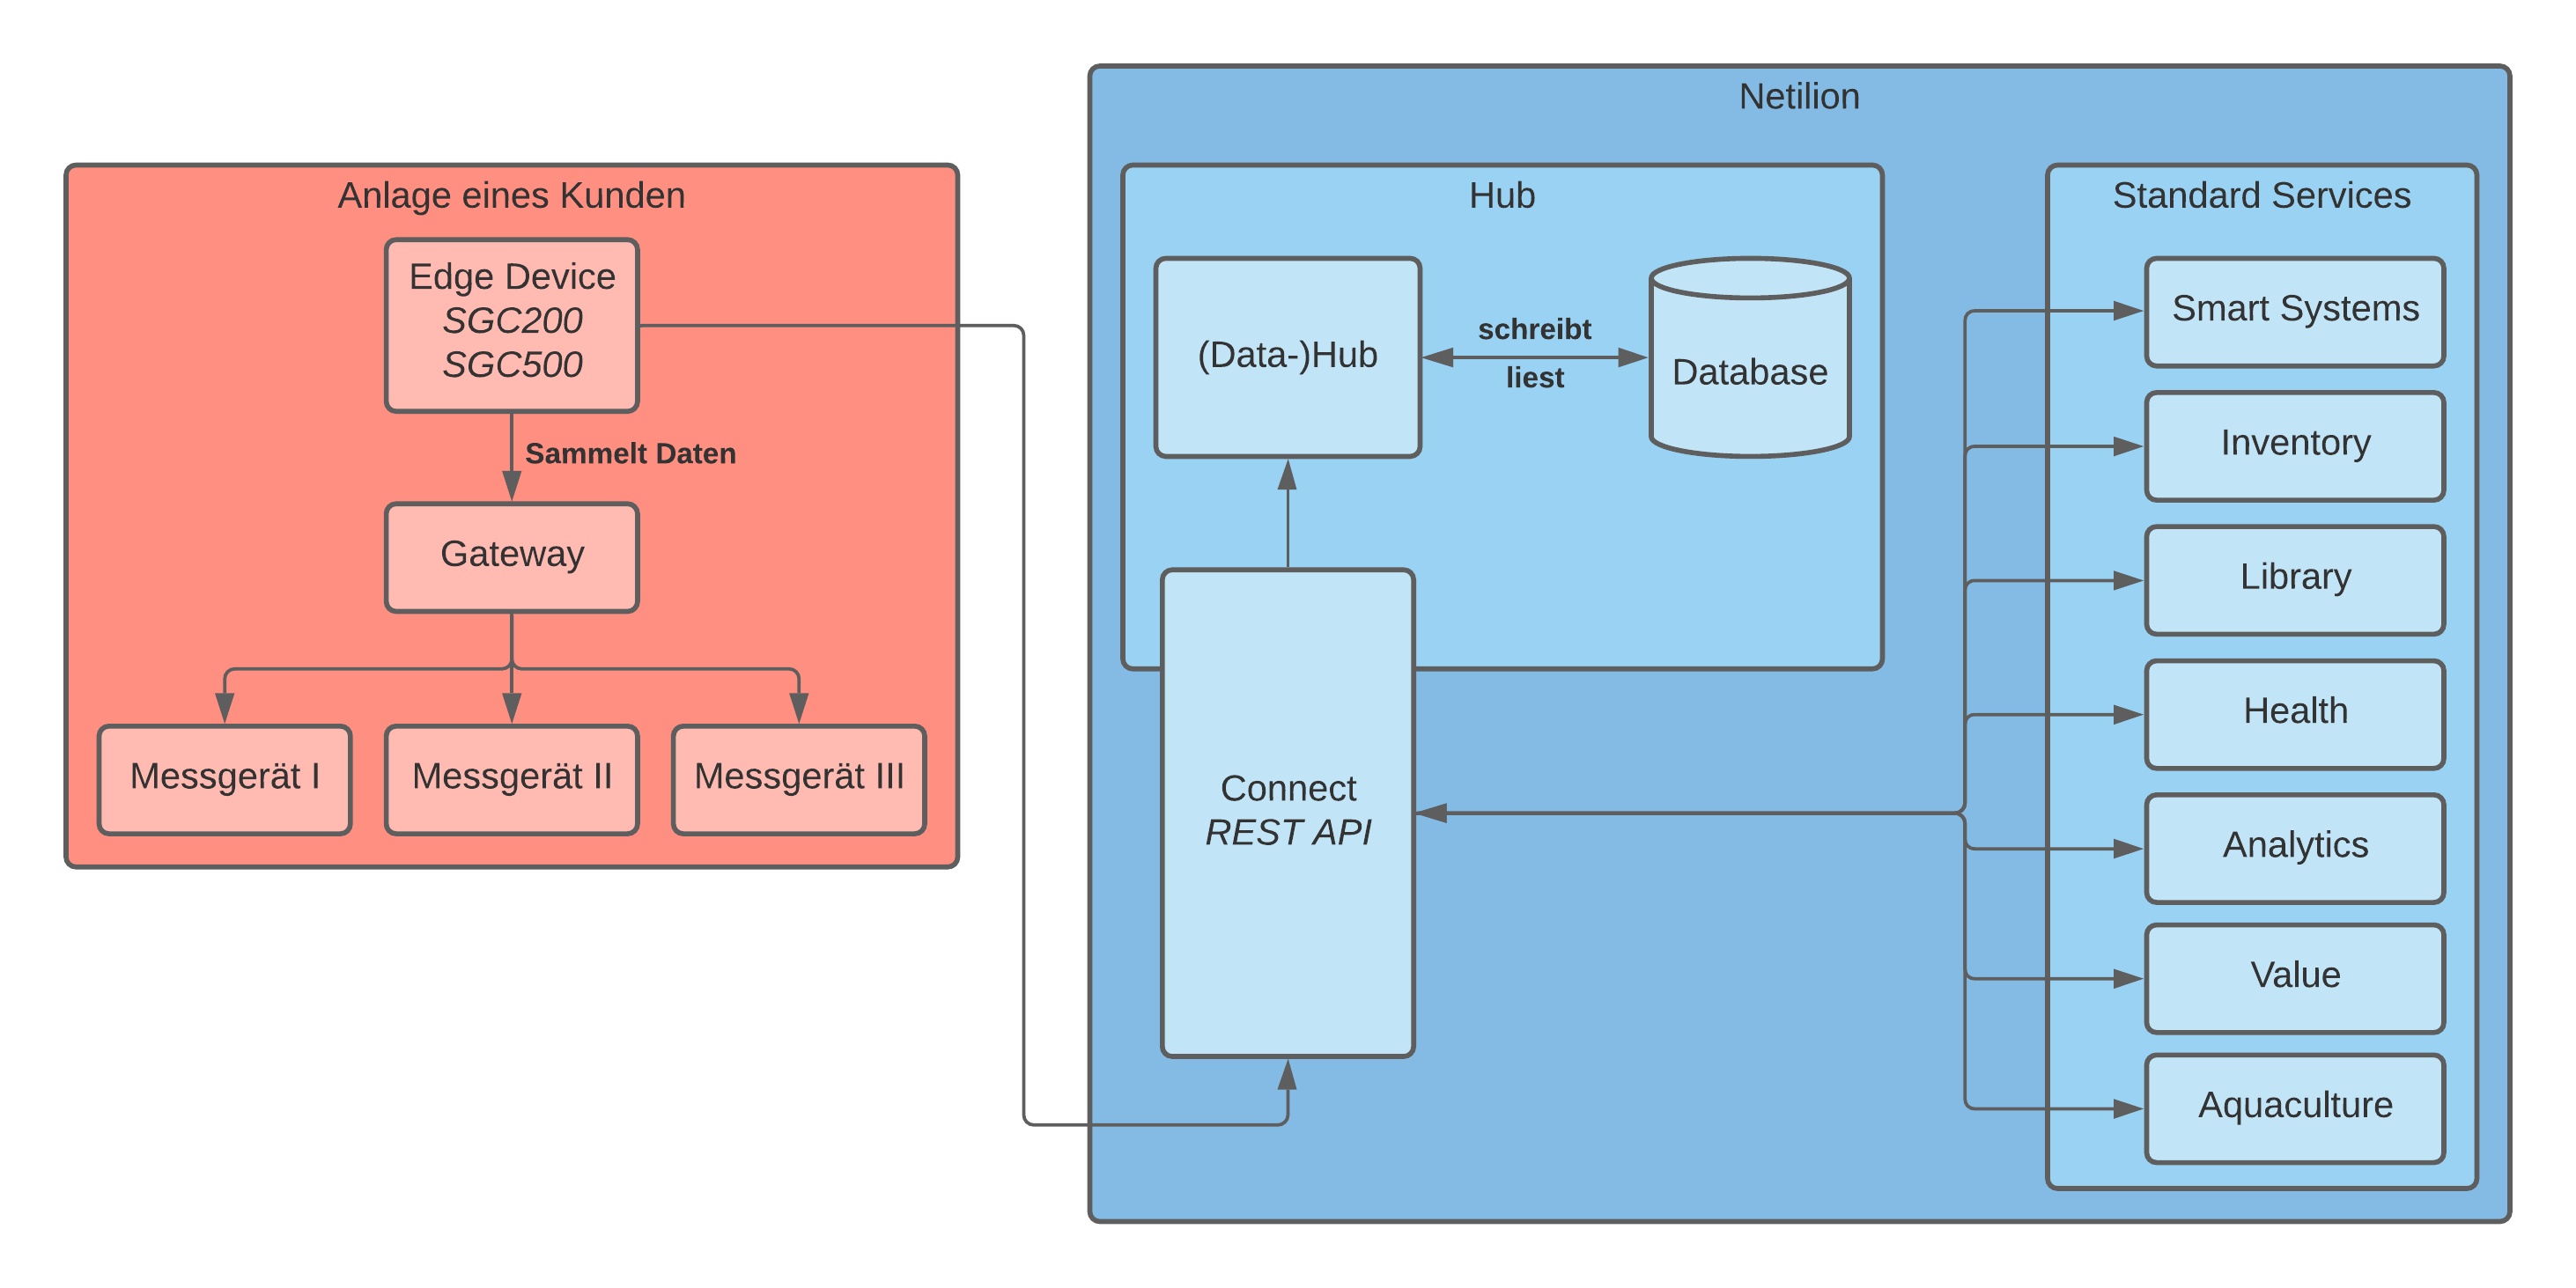
\includegraphics[width=.95\linewidth]{./images/Netilion.png}
  \caption[{Diagram Netilion Ökosystem von Jonas Schultheiss}]{Netilion Ökosystem}
  \label{fig:netilion}
\end{figure}
Netilion ist das IIoT Angebot welches vor einigen Jahren von der Endress+Hauser Digital Solutions ins Leben gerufen wurde. Zuvor hatten Kunden keinen direkten Einblick in die genauen Daten der Messgeräte. Techniker mussten regelmässig vorbei kommen und die Geräte prüfen, auch wenn das Gerät noch optimal lief. Nun ist die ganze Anlage des Kunden ans Internet gebunden, was die Möglichkeiten praktisch grenzenlos macht.
\newline
Die Daten der Messgeräte werden mithilfe eines Edge Devices ausgelesen und zuerst lokal gespeichert. In Intervallen sendet es diese dann an die REST API von Netilion. Da werden sie vom Hub empfangen, validiert und serialisiert. Anschliessend kann der Kunde eine unseren Web Applikationen öffnen und die verarbeiteten Daten grafisch aufbereitet ansehen.
\subsubsection{Hub}
Der Hub ist sozusagen das zentrale Lager aller Daten, welche im Ökosystem verwendet werden. Er bietet die REST API an, validiert Daten, regelt das Benutzer- und Zugriffssystem und speichert das ganze in einer Datenbank.
\subsubsection{Standard Services}
Die Standard Services sind Webapplikationen, welche die Daten der Anlage entgegennehmen, passend darstellt und mit anderen Daten integriert. So zeigt zum Beispiel die Applikation \textit{Health} die NE107 Status der einzelnen Geräte an. \textit{Value} hingegen stellt unter anderem die Messwerte der Geräte dar. Diese Services sind das Herz des IIoT-Angebotes. Sie sollen dem Kunden kosten sparen und Prozesse vereinfachen. 
\subsubsection{Connect}
Netilion Connect ist ein relativ neues Angebot des Ökosystems. Grosse Kunden wollen meist entweder eigene eingekaufte oder von Ihren Entwickler hergestellte Systeme verwenden. Deshalb sollten sie auch ausserhalb unserer Applikation an ihre Daten kommen können können. So ergibt sich zum Beispiel die Möglichkeit ein Dashboard mit den Firmen Guidelines zu erstellen.
\subsection{OSE-Dashboard: Backend} \label{arch-backend}
\begin{figure}[!ht]
  \centering
  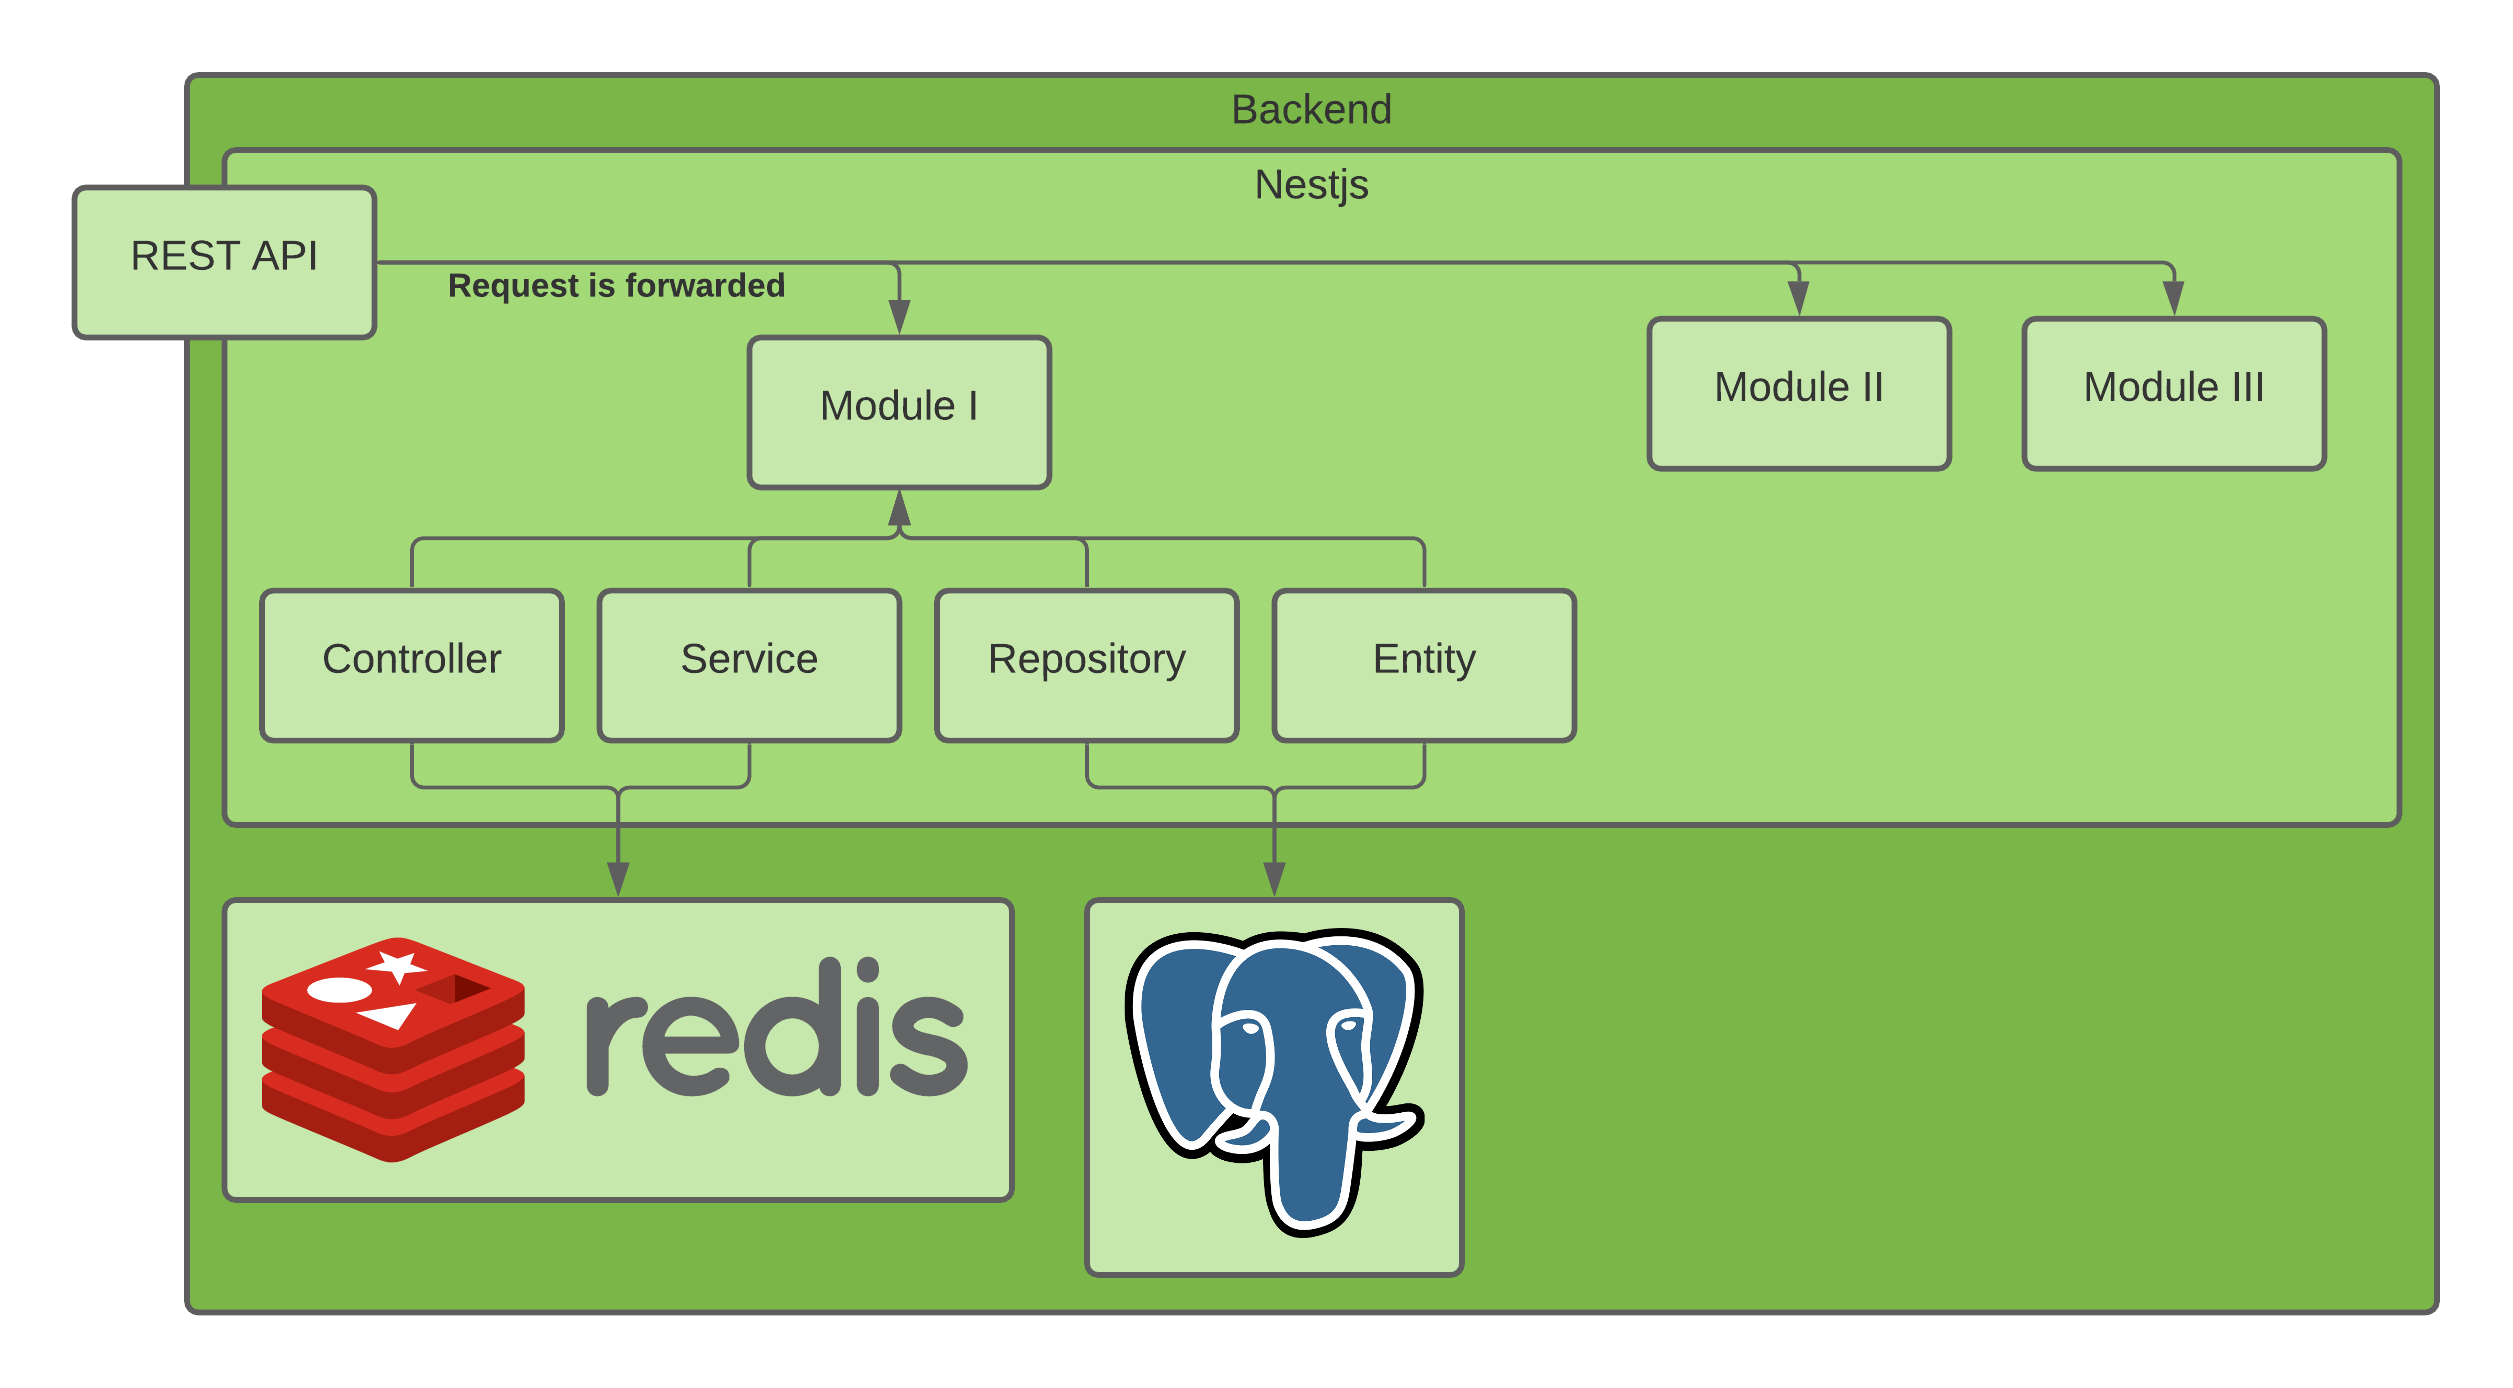
\includegraphics[width=.95\linewidth]{./images/backend.png}
  \caption[{Diagram OSE-Dashboard Backend von Jonas Schultheiss}]{OSE-Dashboard Backend}
  \label{fig:backend}
\end{figure}
Die Aufgabe des Backends war primär das cachen der Daten. Ohne caching hätte jeder Client des Frontends direkt Anfragen an Netilion gesendet. Auch wenn ein Client nur alle 30 Minuten die Daten aktualisiert, wir wissen trotzdem nicht auf wievielen Clients unser Frontend gerade aktiv ist. Das Abonnement der REST-API besitzt eine maximale Nummer an Anfragen welche gemacht werden können, bevor auf das nächst teurere Abonnement aufgerüstet werden muss. Diese Nummer nicht zu überschreiten war ein Kriterium des Product Owners. Da dies schwierig abzuschätzen oder auszurechnen ist mit einer unbekannten Zahl, wurde das Backend erstellt.
\newline
Ein eigenes Backend zu erstellen hat allerdings auch den Vorteil, dass wir zusätztliche Daten anfordern können und diese direkt mit den Netilion Daten verlinken/integrieren können.
\newline
\newline
Kurz vor der IPA hat das Team, welches hinter der Entwicklung von Netilion steht, angekündigt, dass Webhooks nun in der produktion verfügbar sind. Mithilfe von Webhooks kann ein Client einzelne Events abonnieren und erhält direkt bescheid, wenn sich ein Wert ändert. Mit diesen Webhooks müsste ich keine Intervale/Cron jobs verwenden müssen, wodurch die Anzahl der Anfragen deutlich vermindert werden würde.
\newline
Auch wenn ein Lösungsansatz mit Webhooks optimaler wäre, habe ich mich dagegen entschieden es an dieser IPA so zu lösen. Das Feature wurde kurz vor der IPA angekündigt und ich habe bisher keine theoretische oder praktische Erfahrung mit Webhooks. Gerne werde ich es nach dem Abschluss der IPA angehen.
\subsubsection{Nestjs}
Seit dem zweiten Lehrjahr arbeite ich mit JavaScript. Die Sprache hat mich von Anfang an angesprochen. Mit der Hauptgrund war, dass man mit JavaScript nicht nur ein Frontend erstellen kann, sondern mitlerweile dank Nodejs auch Backends/Servers und sogar Apps fürs Smartphone. Wenn ein Produkt im ganzen Stack nur JavaScript verwendet, müssen Entwickler nicht mehrere Sprachen lernen, sondern können sich ganz auf eine Fokussieren, Stücke vom Quellcode können ausgetauscht werden und so weiter.
\newline
Ich habe Erfahrungen mit praktisch allen populären Nodejs Backendframeworks, konnte mich allerdings nie ganz mit einem anfreunden. Die meisten Frameworks sind unopinionated. Dies gefällt mir im Backend nicht, da nach einer relativ kurzen Zeit ein Durcheinander entsteht, welches man dann selber aufräumen kann. Sobald man dann einen passenden Platzt für alles gefunden hat, kann man das gleiche nochmals beim nächsten Projekt wiederholen.
\newline
Nestjs geht komplett in eine andere Richtung. Es ist sehr inspiriert von Java Spring Boot und Angular, ist extrem opinionated und das meiste kommt out-of-the-box, ohne das man selber viele Konfigurierationen machen muss.
\subsubsection{Inspiration}
Wie in Java Spring Boot gibt es Controller, Services, Repositories und Entitäten. Diese werden jeweils nur für eine Resource erstellt. Mögliche Resourcen sind zum Beispiel "users" oder "assets". Wie in Angular werden sie zu einem Modul gebündelt.
\subsubsection{Redis \& Postgresql}
Ich habe mich bei temporärem Caching für Redis entschieden, da ich keine alternative dazu kenne und da es auch sonst intern verwendet wird. Postgresql habe ich genommen, da Netilion und das dahinterstehende Team dies verwendet.
\subsubsection{Hosting}
Das Backend wird auf Heroku gehostet. Gründe dafür sind folgende:
\begin{itemize}
  \item Praktische erfahrung seit dem zweiten Lehrjahr.
  \item Wird intern und bei Netilion verwendet.
  \item Bietet gratis Redis \& Postgresql instanz an, welche für diesen Use-Case komplett ausreichen.
\end{itemize}
\subsection{OSE-Dashboard: Frontend} \label{arch-frontend}
\begin{figure}[!ht]
  \centering
  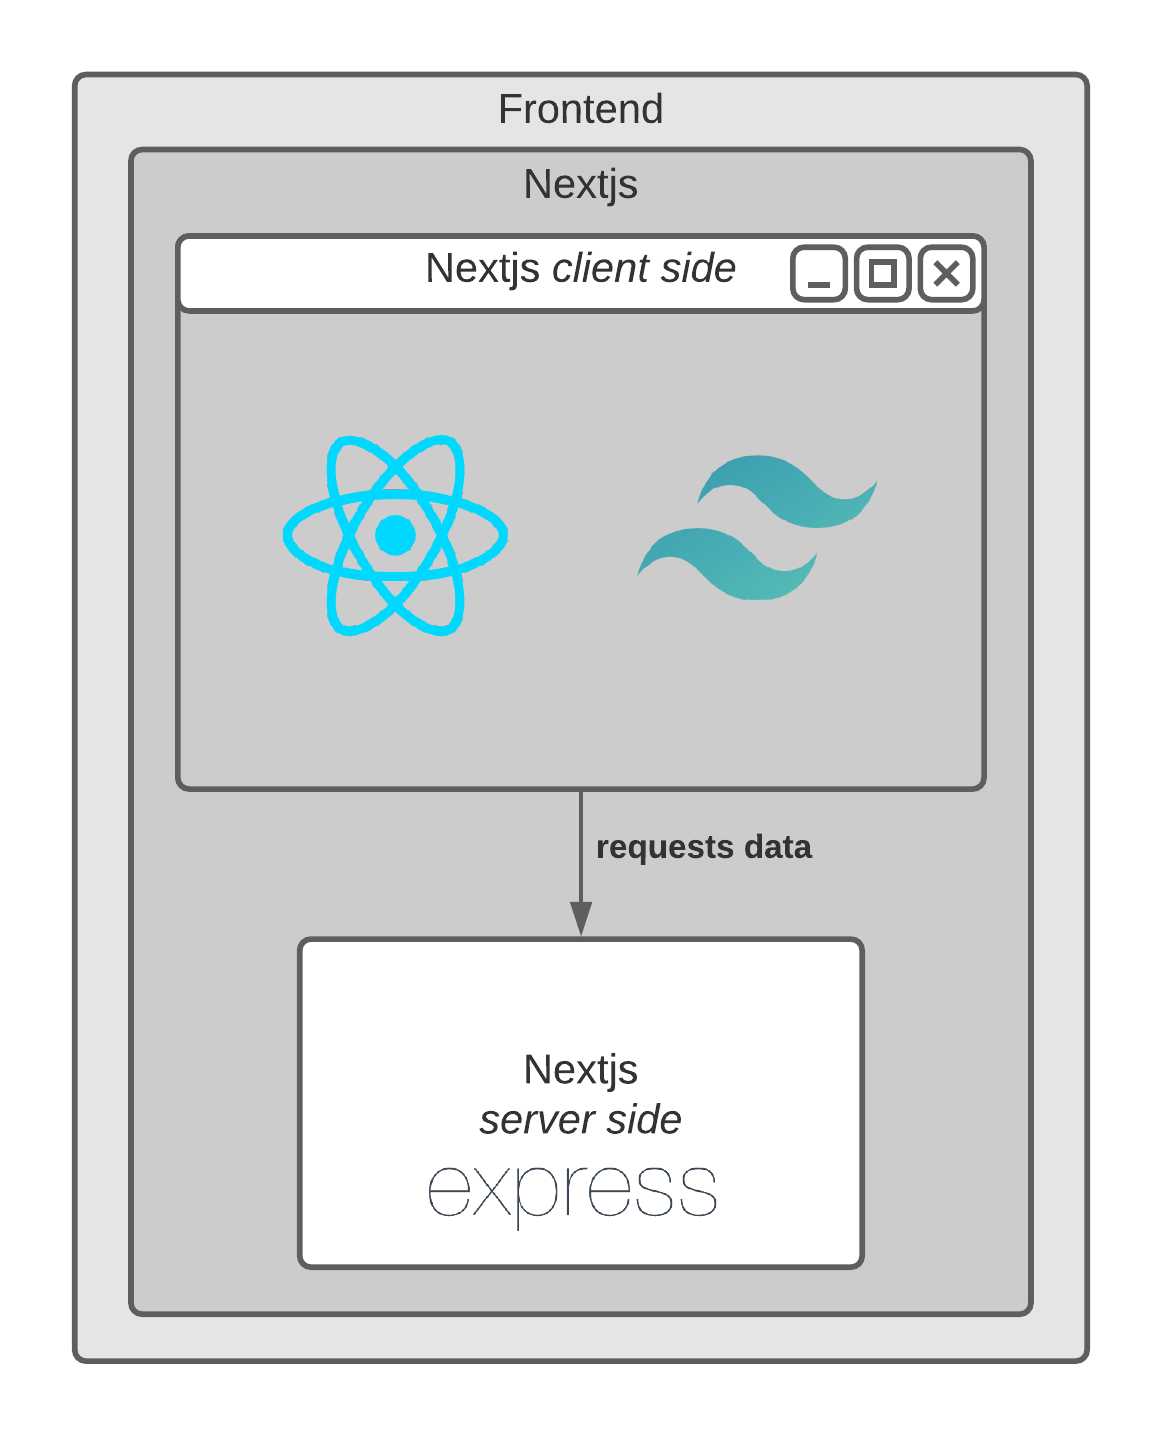
\includegraphics[width=.4\linewidth]{./images/frontend.png}
  \caption[{Diagram OSE-Dashboard Frontend von Jonas Schultheiss}]{OSE-Dashboard Frontend}
  \label{fig:frontend}
\end{figure}
\subsubsection{Hosting}
Das Hosting wird mit Vercel gemacht. Vercel ist eine amerikanische Firma, die sich auf den JAM-Stack fokussiert. Seit 2016 bietet sie eine sehr vereinfachte Möglichkeit moderne JavaScript Frontends zu builden und deployen. Zeitgleich arbeiten sie auch an Nextjs, welches kurze Zeit später veröffentlicht wurde. Nextjs ist ein Frontend Framework, welches routing, server side rendering und viele weitere features mit React verbindet. Nextjs ist für das Hosting auf Vercel optimiert. So ist das Deployment noch einfacher, als bei vergleichbaren Frameworks, und es können tiefere Analysewerte gemessen werden.
\subsubsection{Server Side Rendering}
Eines der Features welches Nextjs ausmacht, ist das server side rendering, welches es out-of-the-box anbietet. So kann man beim entwickeln angeben, welche Seiten statisch und welche dynamisch sein sollen. So wird nicht nur die Erfahrung des Users besser, man steigert auch das SEO ranking. Das Framework baut auf express auf. Dies ermöglicht es einem ein minimales backend in das Frontend einzubauen. Die Vorteile davon sind, dass sensible Daten so nicht beim Benutzer landen.
\section{Ist/Soll-Vergleich}
Ein meiner Meinung nach wichtiger Teil der IPA ist der Vergleich zwischen dem momentan vorhandenen Stand und wie das fertige Produkt aussehen sollte. In den folgenden Kapiteln \ref{ist-zustand} und \ref{soll-zustand} gehe ich auf diese beiden Themen ein.
\subsection{Ist-Zustand} \label{ist-zustand}
\subsubsection{Model}
Bei der Erstellung der Vorarbeit war die verwendung von mehreren Modellen nie ein Thema. Es sollte extra für Reinach angefertigt werden. Zu diesem Zeitpunkt wusste ich sogar nicht einmal, dass die Endress+Hauser Gruppe nochmehr von ihnen besass, geschweige den, dass sie intern standartisiert wurde. Das heisst, dass immer die gleichen Messgeräte auf den Modellen sind.
\newline
Da es sich nur um ein einziges Model handelte, habe ich die ID's der digitalen Zwillingen der Messgeräte per Hand herausgesucht und dann statisch in den Quellcode geschrieben. Dies war der einfachste Weg um das Projekt wie gewünscht umzusetzten. Es gab mir zu diesem Zeitpunkt auch keinen Sinn das ganze dynamisch zu gestalten.
\subsubsection{Credentials}
Damit ich die Daten der Messgeräte erhalten konnte, musste ich credentials verwenden. Dies wurde von Anfang mit Environment Variablen gelöst, da ich leider in der Vergangenheit schon einmal erfahren musste, was es heisst, die Credentials auf GitHub zu pushen. Anfangs wurde dies mit BasicAuth im Server-Side Teil von Nextjs gelöst. Später habe ich es dann allerdings ins Backend verschoben. Momentan verwendet das Projekt noch disen statischen Lösungsweg mit BasicAuth.
\subsubsection{Konfiguration}
Da es sich nur um ein Model handelte, habe ich gewünschte Konfigurationen entweder in Environment Variablen gespeichert oder direkt in den SourceCode geschrieben. Da es nun mehrere Modelle sind, muss unbedingt ein Konfigurationsmenü her.
\subsection{Soll-Zustand} \label{soll-zustand}
\subsubsection{Modelle}
Es sollen nun mehrere Modelle eingebunden werden können und ein User soll zwischen den Standorten wechseln können. Dafür müssen nun neue Entitäten im Backend und neue Tabellen in der Datenbank angelegt werden. Einerseits soll eine \flqq models\frqq Tabelle her, welche die \flqq assets\frqq , also Messgeräte bundelt. Andererseits muss auch der Standord des Models abrufbar sein können, weswegen auch eine \flqq locations\frqq Tabelle erstellt werden sollte.
\subsubsection{OAuth2}
In dieser Erweiterung ist es notwendig, dass sich mehrere Netilion Accounts sicher anmelden können. Ich habe mich in der Vergangenheit sehr intensiv mit OAuth2 beschäftigt und finde, dass ich es optimal für diesen UseCase umsetzten kann. Sprechen wir allerdings über die Entscheidung, wieso OAuth2 verwendet werden sollte und nicht einfach das bestehende BasicAuth Konstrukt erweitert werden sollte.
\begin{itemize}
  \item BasicAuth wird in der nahen Zukunft nicht mehr unterstützt
  \item OAuth2 verbessert wie User Experience, da ein Nutzer nurnoch seinen Login braucht.
  \item OAuth2 vermindert den administrativen Aufwand
  \item Die Lösung ist optimaler und schöner
\end{itemize}
\subsubsection{Konfigurationsmenü}
Damit der Verantwortliche eines OSE Models Einstellungen vornehmen kann, muss unbedingt ein Konfigurationsmenü her. Ein Teil der IPA ist es, die digitalen Zwillinge automatisch mit den Meshes des 3D-Models zu verlinken. Sollte dies aus irgeneinem Grund nicht möglich sein, soll der User dies selbst manuel verlinken können. Damit diese wichtige Einstellung aber nicht von jedem User vorgenommen werden kann, darf nur dies nur ein eingeloggter User, welcher sich in einer Usergroup befindet, vornehmen.
\section{Namenskonzept}
\subsection{User Stories}
\begin{table}[htp]
  \begin{tabularx}{\textwidth}{l l X}\hline \\
  \textbf{Segment} & \textbf{Abkürzung} & \textbf{Beschreibung} \\ \\\hline \\
  1 & US & Abkürzung für User Story \\
  2 & - & Trennzeichen \\
  3 & 01 & Fortlaufende Kennzahl \\
  \\\hline
  \end{tabularx}
\end{table}
\subsection{Akzeptanzkriterien}
\begin{table}[htp]
  \begin{tabularx}{\textwidth}{l l X}\hline \\
    \textbf{Segment} & \textbf{Abkürzung} & \textbf{Beschreibung} \\ \\\hline \\
    1 & AK & Abkürzung für Akzeptanzkriterium \\
    2 & - & Trennzeichen \\
    3 & 01 & Fortlaufende Kennzahl \\
    \\\hline
  \end{tabularx}
\end{table}
\subsection{Test Cases}
\begin{table}[htp]
  \begin{tabularx}{\textwidth}{l l X}\hline \\
  \textbf{Segment} & \textbf{Abkürzung} & \textbf{Beschreibung} \\ \\\hline \\
  1 & TC & Abkürzung für Test Case \\
  2 & - & Trennzeichen \\
  3 & 01 & Fortlaufende Kennzahl \\
  \\\hline
  \end{tabularx}
\end{table}
\subsubsection{Fehlerklassen}
Damit Testergebnisse nach der Prüfung priorisiert werden können, werden ihnen Fehlerklassen zugewiesen.
\newline
Fehlerklassen sind folgenderweise definiert:
\begin{table}[htp]
  \begin{tabularx}{\textwidth}{l l X}\hline \\
  \textbf{Fehlerklasse} & \textbf{Beschreibung} \\ \\\hline \\
  0 & Definiertes Resultat stimmt mit dem getesteten Resultat überein \\
  1 & Definiertes Resultat weicht von dem getestet Resultat ab, beeinträchtigt die \\
    & Funktionalität allerdings nicht \\
  2 & Definiertes Resultat weicht von dem getestet Resultat ab und beeinträchtigt \\
    & die Funktionalität \\
  3 & Definiertes Resultat und getestetes Resultat stimmen nicht überein \\
  \\\hline
  \end{tabularx}
\end{table}
\pagebreak
\subsubsection{Test Case Schema}
\begin{table}[htp]
  \begin{tabularx}{\textwidth}{l l X}\hline \\
  \textbf{Segment} & \textbf{Beschreibung} \\ \\\hline \\
  Name & Name des Testes, gemäss des Namenskonzeptes \\
  Tester & Name der Person, die den Test durchgeführt hat \\
  Erwartetes Resultat & Vom Nutzer gewünschtes Resultat \\
  Effektives Resultat & Eingetroffenes Resultat \\
  Szenario & In Schritten definiertes Testszenario \\
  Fehlerklasse & Zugewiesene Fehlerklasse nach der Überprüfung \\
  Weiteres Vorgehen & Vorgehensbeschreibung, sollte die Fehlerklasse nicht 0 sein \\
  Betroffene Use Cases & Welche Use Cases sind betroffen \\
  Status & Zeigt, ob der Test Case geprüft wurde \\
  \\\hline
  \end{tabularx}
\end{table}
\section{Versionskontrolle}
Ich werde Git mit GitHub verwenden, da ich nun drei Jahre erfahrung damit habe und mein Lehrbetrieb die gleiche Strategie verfolgt. Dabei werde ich immer nach Abschluss eines Abschnittes einen Commit erstellen. Wichtig ist, dass der Master Branch immer problemlos läuft und deployed werden kann.
\newline
\newline
Diese IPA ist in drei Teile aufgebrochen: das Frontend, das Backend und die Dokumentation. Für alle drei Teile verwende ich Git \& GitHub. Hier ist eine auflistung aller Repositories:
\begin{table}[htp]
  \begin{tabularx}{\textwidth}{l X}
  Frontend: & \href{https://github.com/EndressHauser-ProcessSolutions/ose-dashboard-frntnd}{EndressHauser-ProcessSolutions/ose-dashboard-frntnd} \\
  Backend: & \href{https://github.com/EndressHauser-ProcessSolutions/ose-dashboard-bcknd}{EndressHauser-ProcessSolutions/ose-dashboard-bcknd} \\
  Dokumentation & \href{https://github.com/EndressHauser-ProcessSolutions/ose-dashboard-docs}{EndressHauser-ProcessSolutions/ose-dashboard-docs} \\
  \end{tabularx}
\end{table}
\subsection{Git Flow}
\begin{figure}[!ht]
  \centering
  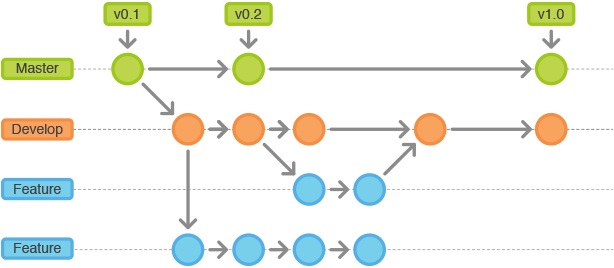
\includegraphics[width=0.8\linewidth]{./images/Gitflow-Workflow-2.png}
  \caption[\href{https://blog.ordix.de/welches-vorgehen-eignet-sich-fuer-mein-projekt}{Grafik, welche den Git Flow arbeitsablauf visualisiert}]{Git Flow visualisiert}
  \label{fig:git-flow}
\end{figure}
Mit dem Git Flow definiert ein Team oder ein Entwickler, wie sie/er die Versionskontrolle in Git handhabt. Es gibt drei Arten von Branches:
\begin{itemize}
  \item \textbf{Master} - Enthält immer die lauffähige und stabile Version, welche gerade deployed ist.
  \item \textbf{Develop} - Dies ist der Branch, auf dem Entwickelt wird. Er soll immer lauffähig sein, damit neue Features getestet werden können, bevor sie zum Master gemerged werden.
  \item \textbf{Feature} - Die Einzelnen Stories und Tasks werden in einem Feature Branch entwickelt. Sobald das Feature fertig ist, kann es in den Develop Branch gemerged werden.
\end{itemize}
Diese Strategie bietet einige Vorteile:
\begin{itemize}
  \item Der Master Branch kann mithilfe von CI/CD automatisch deployed werden. So erreichen neue Features schneller den Kunden
  \item Der Develop Branch kann auch mit CI/CD automatisch deployed werden, damit features intern einfacher und schneller besprochen werden können.
  \item Durch die klare Abtrennung dieser Branches erhöht sich die Stabilität der Software, was die Kundenzufriedenheit erhöht.
  \item Features können abgekapselt entwickelt werden.
  \begin{itemize}
    \item Develop Branch bleibt dadurch immer lauffähig
    \item Mehrere Features können gleichzeitig entwickelt werden, ohne sich in die Quere zu kommen
    \item Bietet bessere Übersicht auf GitHub
  \end{itemize}
\end{itemize}
\subsection{Pipelines zu Vercel und Heroku}
Vercel und Heroku bieten Build-Pipelines an. Mit diesen kann ein Branch mit Vercel oder Heroku verbunden werden. Wird ein neuer Commit gepusht, triggert dies den Buildprozess von Vercel oder Heroku, woraufhin man kurze Zeit später eine Live Version hat.
\newline
\newline
Ich werde jeweils zwei Pipelines einrichten. Einmal die Produktionsumgebung mit dem Master Branch und einmal die Testumgebung mit dem Develop Branch.
\subsection{Dokumentation}
Die Dokumentation ist in LaTeX geschrieben und wird regelmässig auf GitHub in ein separates Repository gepusht. Im GitHub habe ich ausserdem ein GitHub Action eingerichtet, welche nach jedem push getriggert wird, das Dokument als pdf rendert und zum Download zur verfügung stellt.
\newline
\newline
Bei der Versionierung dieses Dokumentes orientiere ich mich an meiner Einschätzung verbunden mit folgendem System:
\begin{table}[htp]
  \begin{tabularx}{\textwidth}{l l X}\hline \\
  \textbf{Versionsartefakt} & \textbf{Beispiel} & \textbf{Beschreibung} \\ \\\hline \\
  1 & 0 & \textbf{Major} Grosse Abschlüsse des Dokumentes \\
  2 & . & Trennzeichen \\
  3 & 1 & \textbf{Minor} Eine Änderung wie z.B. ein neues Kapitel \\
  4 & . & Trennzeichen \\
  5 & 3 & \textbf{Patch} Kleine änderung / Neue Texte in einem Kapitel \\
  \\\hline
  \end{tabularx}
\end{table}
\newline
Wichtig zu beachten ist, dass ich bei der Dokumentation \textbf{nicht GitFlow einsetzte}, da es keinen Vorteil für den Aufwand bietet.
\section{Backupkonzept}
Die ganze Dokumentation und jeglicher Code wird mindestens einmal Täglich auf GitHub gepusht. Optimal ist, wenn der Code im Falle vom Front- und Backend nach jedem Feature gepusht wird und bei der Dokumentation nach der fertigstellung eines Unterkapitels. Sollte was verloren gehen kann man so also immer mindestens auf den letzten Stand des Vorabends zurückzuspringen.
\newline
\newline
Das MacBook wird mithilfe vom vorinstallierten Tool \flqq Time Machine\frqq ständig inkrementell auf einer externen SSD gesichert. Time Machine speichert dabei folgendes \cite{apple_2021_mit}:
\begin{itemize}
  \item Lokale Schnappschüsse, solange Speicherplatz vorhanden ist
  \item Stündliche Backups der letzten 24 Stunden
  \item Tägliche Backups des letzten Monats
  \item Wöchentliche Backups aller vorherigen Monate
\end{itemize}
Somit ist eine schnelle weiterarbeit trotz Hardwareproblemen möglich.
\subsection{Sicherheit der Daten}
Die Repositories befinden sich auf dem GitHub Team der Firma. Dieses Team ist so sicher eingerichtet, wie es GitHub erlaubt. Meine Accounts verwenden beide sichere Passwörter und Two-Way-Authentificator.
\newline
Die interne SSD des MacBooks \cite{a2021_hardware} und die externe SSD \cite{a2021_keep} sind verschlüsselt.
\section{Personas}
\begin{figure}[!ht]
  \centering
  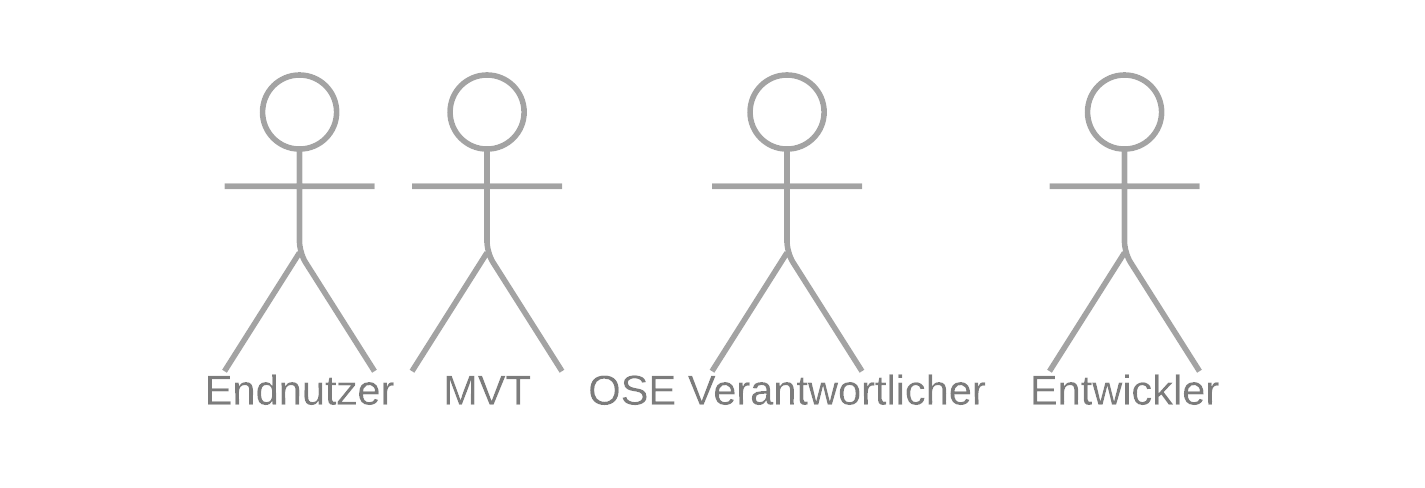
\includegraphics[width=0.6\linewidth]{./images/Personas.png}
  \caption[Personas]{Personas}
  \label{fig:personas}
\end{figure}
\subsection{Endnutzer}
Der Endnutzer ist schlussendlich der Besucher, welcher am Fernseher mit dem Dashboard interagiert. Er möchte möglich einfach die Daten des OSE-Models ansehen können, ohne sich dabei einloggen zu müssen.
\subsection{MVT}
Das MVT Team ist für interne und externe Trainings unseres Portfolios zuständig. Markus Reisgis von MVT war der originale Auftraggeber. Für sie ist wichtig, dass alle gewünschten Daten korrekt angezeigt werden und das der Endnutzer eine gute Erfahrung macht.
\subsection{OSE Verantwortlicher}
Der OSE Verantwortliche ist die Person, welche für ein Model verantwortlich ist. Dies ist zum Beispiel MVT in Reinach. Es gibt allerdings noch einige weitere in Deutschland, Frankreich und so weiter. Für sie ist wichtig, dass sie wenig Mehraufwand haben. Im optimalen Fall sollte Login und die eventuelle Konfiguration möglichts einfach und fehlerfrei ablaufen.
\subsection{Entwickler}
Der Entwickler bin ich. Mir ist es wichtig, alle gewünschten Features kompetent und wie gewünscht umzusetzten, und dabei den Fortschritt korrekt zu dokumentieren.
\section{User Stories}
\subsection{US-01}
Als OSE Verantwortlicher möchte ich mich einloggen können, damit ich mein Model registrieren kann.
\begin{itemize}
  \item AK-01 Login möglich
  \item AK-02 Login Daten sind geschützt und nicht von einem Benutzer auslesbar
  \item AK-03 Bei einem Fehlversuch wird eine passende Fehlermeldung angezeigt
  \item AK-04 Es gibt eine unlimitierte anzahl an 
\end{itemize}
\subsection{US-02}
Als OSE Verantwortlicher möchte ich, dass die digitalen Zwillinge der Messgeräte automatisch verlinkt werden, ohne das ich etwas machen muss, solange sie standartisiert sind.
\begin{itemize}
  \item AK-01 Automatische verlinkung bei Registrierung funktioniert, solange die Assets nach dem Standard benannt sind
  \item AK-02 Methode, welche die Verlinkung vornimmt ist mit automatischen Tests abgedeckt
\end{itemize}
\subsection{US-03}
Als OSE Verantwortlicher möchte ich ein Konfigurationsmenü, mit welchem ich die V§erlinkung manuel ändern kann, sollte ich ein Gerät austauschen.
\begin{itemize}
  \item AK-01 Konfigurationsmenü ist aufrufbar
  \item AK-02 Verlinkungen sind manuel veränderbar
\end{itemize}
\subsection{US-04}
Als OSE Verantwortlicher möchte ich sicher sein, dass kein Endnutzer die Verlinkung ändern kann.
\begin{itemize}
  \item AK-01 Konfigurationsmenü ist nur aufrufbar, solange der OSE Verantwortliche eingeloggt ist
  \item AK-02 Konfigurationsmenü ist nur aufrufbar, solange sich der Account in einer spezifischen User Gruppe befindet
\end{itemize}
\subsection{US-05}
Als Endnutzer möchte ich die Applikation nutzen können, ohne mich einloggen zu müssen.
\begin{itemize}
  \item AK-01 Applikation ist weiterhin ohne Login nutzbar
\end{itemize}
\subsection{US-06}
Als Endnutzer möchte ich die Datenquelle des OSE-Dashboards aus den verfügbaren Standorten auswählen können, damit ich auch Daten anderer Modelle sehen kann.
\begin{itemize}
  \item AK-01 Standort kann geändert werden
  \item AK-02 Übersicht über alle verfügbaren Standorte ist implementiert
\end{itemize}
\section{OAuth2 Strategie}
\subsection{Was ist OAuth2?}
OAuth2 wurde ins Leben gerufen, um einen spezifischen UseCase zu decken. Eine Applikation eines Drittanbieters möchte zum Beispiel Daten des Users von Spotify abrufen. Vor OAuth2 musste der User seine Logindaten an den Drittanbieter senden, welcher diese dann in Klartextformat abspeichern musste, damit er später selber die Daten abrufen kann.
\newline
Der User hatte so keine Kontrolle über die Aufbewahrung der Logindaten und wusste schon garnicht was der Drittanbieter alles mit den Logindaten anstellt. Zusammengefasst war der ganze Prozess sehr unsicher und der User übergab immer alle Rechte des Accounts.
\newline
\newline
Mit OAuth2 konnte dieser Prozess nun sicher gestaltet werden. Der User wird auf die Anmeldeseite des OAuth2-Providers weitergeleitet und meldet sich dort an. So kommt die Applikation des Drittanbieters zu keinem Zeitpunkt an die Logindaten. Als nächstes wird dem User gezeigt, auf was für Daten der Drittanbieter zugriff haben möchte. Akzeptiert der User, wird er wieder zurück an den Drittanbieter weitergeleitet, welcher mit diesem Schritt einen Zugriffstoken erhält. Dieser ist nur von dieser Applikation und auf diesen User nutzbar, um die Daten, die der User freigegeben hat, anzufragen.
\pagebreak
\subsection{Anwendung im OSE-Dashboard}
\begin{figure}[!ht]
  \centering
  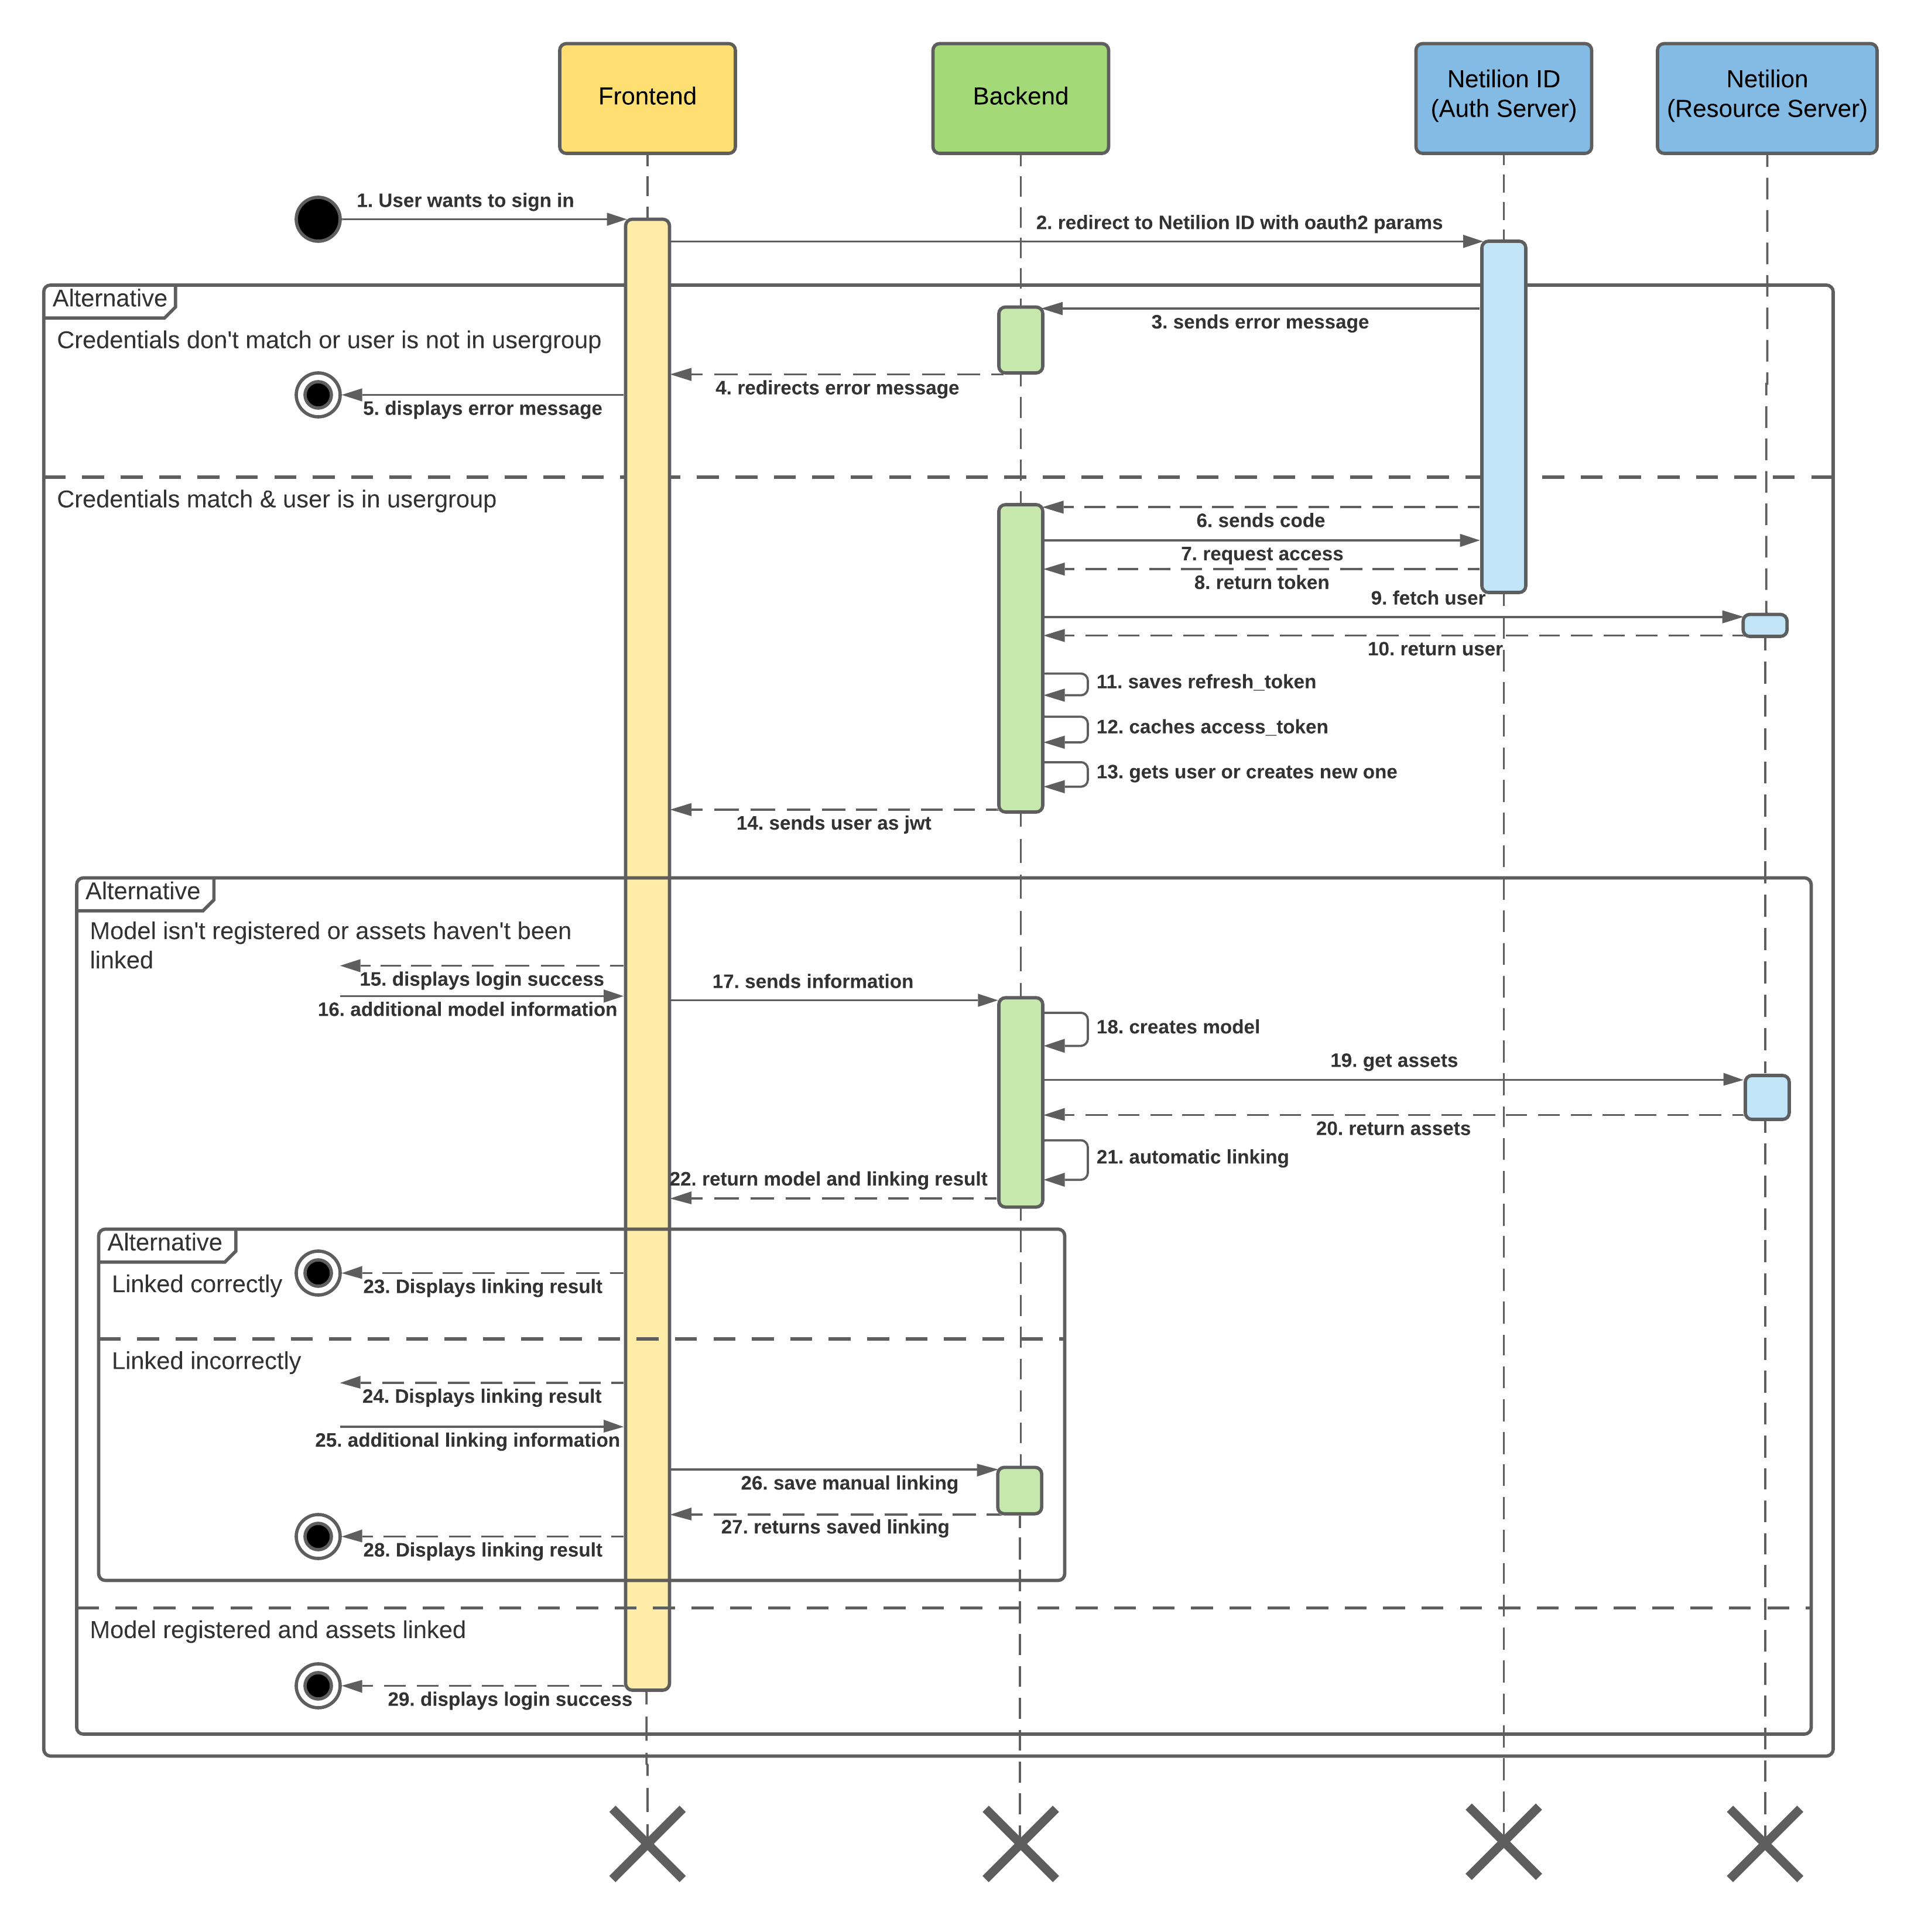
\includegraphics[width=1\linewidth]{./images/OAuth2.png}
  \caption[OAuth2 visualisiert durch ein Sequenzdiagram]{OAuth2 visualisiert durch ein Sequenzdiagram}
  \label{fig:oauth2}
\end{figure}
Folgend ist eine Auflistung der einzelnen Schritte, welche in der Abbildung \ref{fig:oauth2} dargestellt sind.
\begin{enumerate}
  \item Der User will sich einloggen und klickt auf ein \code{<a></a>} tag.
  \item Daraufhin wird er zu Netilion ID weitergeleitet. Die URL enthält dabei die \code{client\_id} und \newline\code{redirect\_uri}. Dadurch weiss Netilion, welche Applikation die Anfrage macht und wohin der User nach der Anmeldung weitergeleitet werden möchte.
  \item Gibt es ein Problem mit dem Login, erhält die \code{redirect uri}, also unser Backend, eine Fehlermeldung.
  \item Mit dieser Fehlermeldung in der URl wird der User wieder ans Frontend weitergeleitet.
  \item Das Frontend nimmt die Fehlermeldung entgegen und stellt sie für den User dar.
  \item Wenn alles korrekt ablauft, erhält unser Backend einen Code.
  \item Mit diesem Code kann das Backend dann einen Zugriffstoken anfordern.
  \item Dieser wird von Netilion ID an unser Backend geschickt.
  \item Mit diesem Zugriffstoken ist es dann möglich Daten von Netilion abzufragen, in diesem Fall der User.
  \item Die Daten des Users werden anschliessend zurückgeschickt.
  \item Der \code{refresh\_token} wird encrypted und in der Datenbank gespeichert.
  \item Der \code{access\_token} wird in redis gecached.
  \item Existiert der User, wird dieser aus der Datenbank gelesen. Existiert er nicht wird ein neuer erstellt.
  \item Der User wird als JWT zurück ans Frontend geschickt.
  \item Das Frontend zeigt an, dass die Anmeldung erfolgreich verlief.
  \item Wenn das Model noch nicht registriert wurde oder die Messgeräte noch nicht verlinkt wurden, wird der User nach zusätzlichen Daten, wie dem Standort, gefragt.
  \item Das Frontend schickt diese Daten mit dem JWT an das Backend.
  \item Das Backend erstellt ein neues Model mit den Daten des Users.
  \item Anschliessend fragt es bei Netilion nach allen Messgeräten nach.
  \item Netilion antwortet mit allen Messgeräten des Users.
  \item Daraufhin erfolgt die automatische Verlinkung.
  \item Das Model mitsamt verlinkten Messgeräten wird ans Frontend weitergeleitet.
  \item Stimmt die Verlinkung ist der Nutzer zufrieden und der Prozess beendet.
  \item Stimmt die Verlinkung nicht, da der Nutzer nicht die standartisierten Geräte oder benennungen verwendet, wird ihm das Resultat angezeigt.
  \item Daraufhin verlinkt der User selbst die Geräte.
  \item Dies wird ans Backend gesendet, damit die Änderungen gespeichert werden können.
  \item Die gespeicherten Änderungen werden an das Frontend geschickt.
  \item Der User wird benachrichtigt, dass seine Änderungen übernommen wurden. Der User ist zufrieden und der Prozess beendet.
  \item Ist das Model bereits registriert und die Messgeräte verlinkt, ist der Prozess beendet.
\end{enumerate}
